\documentclass[8pt]{article}
\usepackage[UTF8]{ctex}
\usepackage[a4paper]{geometry}

\usepackage{amsthm,amsmath,amssymb}
\usepackage{graphicx}
\usepackage{subfigure}
\usepackage{amsmath}
\usepackage{tabularx}
\usepackage{color}
\usepackage{hyperref}
\usepackage{ulem}
\usepackage{multirow}
\usepackage[cache=false]{minted}
\hypersetup{
	colorlinks=true,
	linkcolor=blue
}

\usepackage{appendix}
\geometry{a4paper,centering,scale=0.8}
\geometry{left=2.0cm, right=2.0cm, top=2.5cm, bottom=2.5cm}
\usepackage[format=hang,font=small,textfont=it]{caption}
\usepackage[nottoc]{tocbibind}

\usepackage{algorithm}
\usepackage{algorithmicx}
\usepackage{algpseudocode}
\usepackage{amssymb}
\usepackage{extarrows}
\usepackage{qcircuit}
\usepackage{fancyhdr}
\usepackage{cleveref}
\usepackage{totpages}
\usepackage{pgf}
\usepackage{tikz}
\usepackage{bbm}
\usepackage{tikz}

\usetikzlibrary{arrows,automata}
\usetikzlibrary{arrows.meta}%画箭头用的包
\tikzset{
->, % makes the edges directed
>=stealth', % makes the arrow heads bold
node distance=2.5cm, % specifies the minimum distance between two nodes. Change if necessary.
every state/.style={thick, fill=gray!10}, % sets the properties for each ’state’ node
initial text=$ $, % sets the text that appears on the start arrow
}
\makeatletter
\def\@maketitle{%
	\newpage
	\begin{center}%
		\let \footnote \thanks
		{\LARGE \@title \par}%
		\vskip 1.5em%
		{\large
			\lineskip .5em%
			\begin{tabular}[t]{c}%
				\@author
			\end{tabular}\par}%
		\vskip 1em%
		{\large \@date}%
	\end{center}%
	\par
	\vskip 1.5em}
\makeatother

\newtheoremstyle{compact}%
{3pt}{3pt}%
{}{}%
{\bfseries}{\textcolor{red}{.}}%  % Note that final punctuation is omitted.
{.5em}{\mbox{\textcolor{red}{\thmname{#1}\thmnumber{ #2}}\thmnote{ (\textcolor{blue}{#3})}}}
\theoremstyle{compact}
\newtheorem{innercustomgeneric}{\customgenericname}
\providecommand{\customgenericname}{}
\newcommand{\newcustomtheorem}[2]{%
	\newenvironment{#1}[1]
	{%
		\renewcommand\customgenericname{#2}%
		\renewcommand\theinnercustomgeneric{##1}%
		\innercustomgeneric
	}
	{\endinnercustomgeneric}
}

\DeclareMathOperator{\card}{card}

\newtheorem{theorem}{定理}
\newtheorem{lemma}{引理}
\newtheorem{definition}{定义}
\newtheorem{proposition}{命题}
\newtheorem{corollary}{推论}
\newtheorem{remark}{注}
\newtheorem{Proof}{证明}

\def\obj#1{\textbf{\uline{#1}}}
\def\num#1{\textnormal{\textbf{\mbox{\textcolor{blue}{(#1)}}}}}
\def\le{\leqslant}
\def\ge{\geqslant}
\def\im{\text{im }}
\def\Pr#1{\text{Pr}\left[{#1}\right]}
\def\E#1{\mathbb{E}\left[{#1}\right]}
\def\Var#1{\text{Var}\left[{#1}\right]}


\title{\heiti\zihao{1} 编译原理 \ 第二次作业}
\author{\kaishu\zihao{-3} 周书予\\2000013060@stu.pku.edu.cn}

\CTEXoptions[today=old]
\date{\today}

\begin{document}
\fancypagestyle{plain}{
	\fancyhf{}
	\lhead{编译原理}
	\chead{2022 Spring}
	\rhead{第二次作业}
	\cfoot{第 \thepage 页, 共 \pageref{TotPages} 页}
}
\pagestyle{plain}



\crefname{theorem}{定理}{定理}
\crefname{lemma}{引理}{引理}
\crefname{figure}{图}{图}
\crefname{table}{表}{表}	
\maketitle
\section*{1}
\begin{center} % ’ht’ tells LaTeX to place the figure ’here’ or at the top of the page
	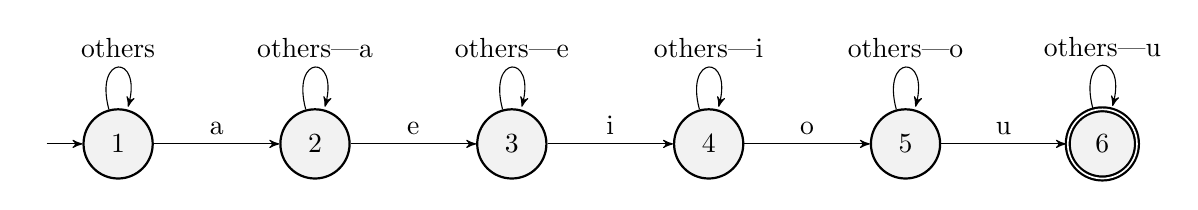
\begin{tikzpicture}
		\node[state, initial] (1) {1};
		\node[state, right of=1] (2) {2};
		\node[state, right of=2] (3) {3};
		\node[state, right of=3] (4) {4};
		\node[state, right of=4] (5) {5};
		\node[state, right of=5, accepting] (6) {6};
		\draw (1) edge[above] node {a} (2)
			(2) edge[above] node {e} (3)
			(3) edge[above] node {i} (4)
			(4) edge[above] node {o} (5)
			(5) edge[above] node {u} (6)
			(1) edge[loop above] node {others} (1)
			(2) edge[loop above] node {others|a} (2)
			(3) edge[loop above] node {others|e} (3)
			(4) edge[loop above] node {others|i} (4)
			(5) edge[loop above] node {others|o} (5)
			(6) edge[loop above] node {others|u} (6);
	\end{tikzpicture}
\end{center}
其中 others $\rightarrow$ [b-d|f-h|j-n|p-t|v-z].

\section*{2}
\begin{center}% ’ht’ tells LaTeX to place the figure ’here’ or at the top of the page
	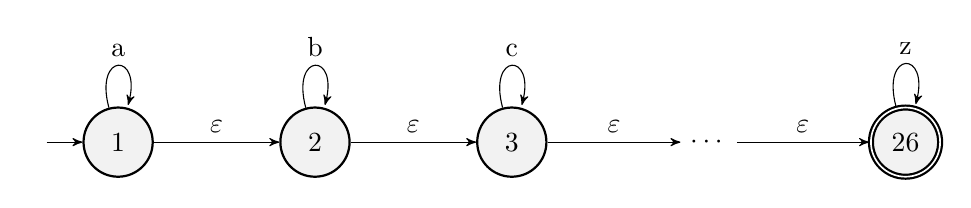
\begin{tikzpicture}
		\node[state, initial] (1) {1};
		\node[state, right of=1] (2) {2};
		\node[state, right of=2] (3) {3};
		\node[right of=3] (4) {$\cdots$};
		\node[state, right of=4, accepting] (5) {26};
		\draw (1) edge[above] node {$\varepsilon$} (2)
			(2) edge[above] node {$\varepsilon$} (3)
			(3) edge[above] node {$\varepsilon$} (4)
			(4) edge[above] node {$\varepsilon$} (5)
			(1) edge[loop above] node {a} (1)
			(2) edge[loop above] node {b} (2)
			(3) edge[loop above] node {c} (3)
			(5) edge[loop above] node {z} (5);
	\end{tikzpicture}
\end{center}

\section*{3}
\begin{center} % ’ht’ tells LaTeX to place the figure ’here’ or at the top of the page
	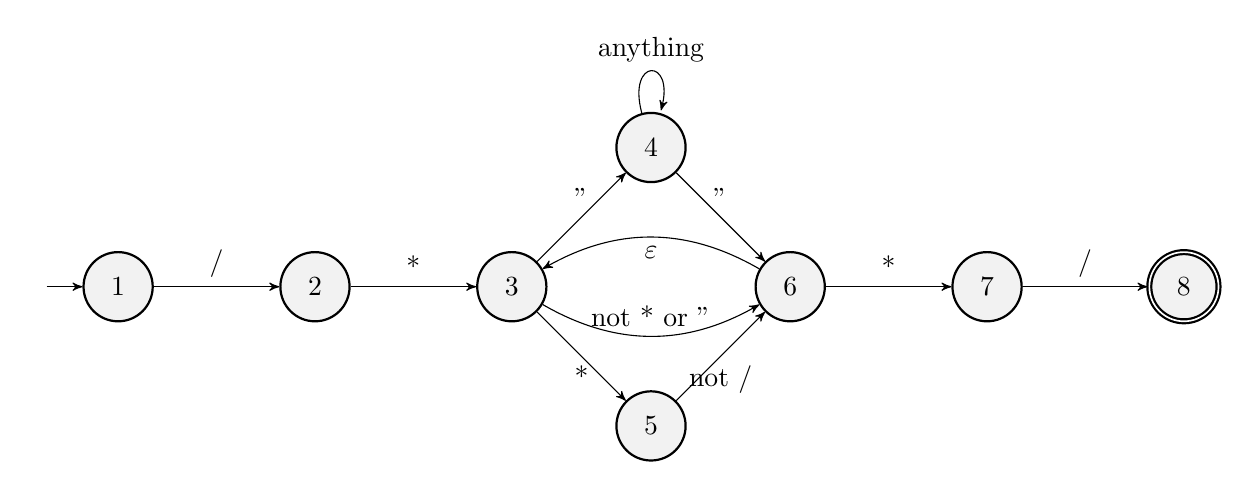
\begin{tikzpicture}
		\node[state, initial] (1) {1};
		\node[state, right of=1] (2) {2};
		\node[state, right of=2] (3) {3};
		\node[state, above right of=3] (4) {4};
		\node[state, below right of=3] (5) {5};
		\node[state, below right of=4] (6) {6};
		\node[state, right of=6] (7) {7};
		\node[state, accepting, right of=7] (8) {8};

		\draw (1) edge[above] node {/} (2)
			  (2) edge[above] node {*} (3)
			  (3) edge[above] node {"} (4)
			  (4) edge[loop above] node {anything} (4)
			  (4) edge[above] node {"} (6)
			  (3) edge[below] node {*} (5)
			  (5) edge[below] node {not /} (6)
			  (3) edge[above, bend right] node {not * or "} (6)
			  (6) edge[below, bend right] node {$\varepsilon$} (3)
			  (6) edge[above] node {*} (7)
			  (7) edge[above] node {/} (8);
	\end{tikzpicture}
\end{center}

\section*{6}
\begin{center} % ’ht’ tells LaTeX to place the figure ’here’ or at the top of the page
	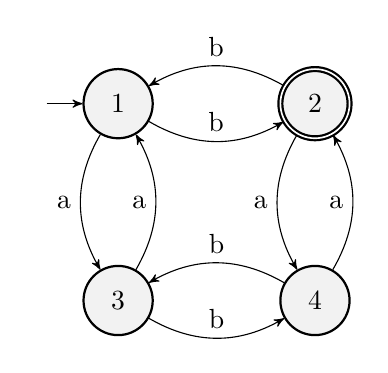
\begin{tikzpicture}
		\node[state, initial] (1) {1};
		\node[state, right of=1, accepting] (2) {2};		
		\node[state, below of=1] (3) {3};
		\node[state, right of=3] (4) {4};		
		\draw (1) edge[above, bend right, left=0.3] node {a} (3) 
			(3) edge[above, bend right, left=0.3] node {a} (1) 
			(2) edge[above, bend right, left=0.3] node {a} (4) 
			(4) edge[above, bend right, left=0.3] node {a} (2)

			(1) edge[above, bend right, above=0.3] node {b} (2)
			(2) edge[above, bend right, above=0.3] node {b} (1)
			(3) edge[above, bend right, above=0.3] node {b} (4)
			(4) edge[above, bend right, above=0.3] node {b} (3);

	\end{tikzpicture}
\end{center}

\section*{9}
\begin{center} % ’ht’ tells LaTeX to place the figure ’here’ or at the top of the page
	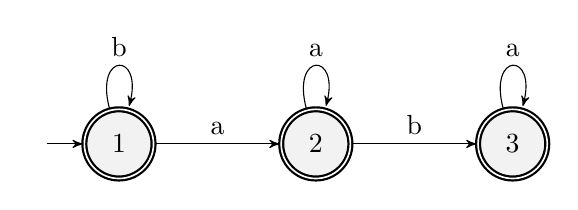
\begin{tikzpicture}
		\node[state, initial, accepting] (1) {1};
		\node[state, right of=1, accepting] (2) {2};
		\node[state, right of=2, accepting] (3) {3};
%		\node[state, right of=3,] (4) {4};
		\draw (1) edge[above] node {a} (2)
		(2) edge[above] node {b} (3)
%		(3) edge[above] node {b} (4)
		(1) edge[loop above] node {b} (1)
		(2) edge[loop above] node {a} (2)
		(3) edge[loop above] node {a} (3);
	\end{tikzpicture}
\end{center}


%\begin{center}
%	\includegraphics*[scale=0.21]{0308.jpg}
%\end{center}

\end{document}
